\documentclass[]{article}
\usepackage{lmodern}
\usepackage{amssymb,amsmath}
\usepackage{ifxetex,ifluatex}
\usepackage{fixltx2e} % provides \textsubscript
\ifnum 0\ifxetex 1\fi\ifluatex 1\fi=0 % if pdftex
  \usepackage[T1]{fontenc}
  \usepackage[utf8]{inputenc}
\else % if luatex or xelatex
  \ifxetex
    \usepackage{mathspec}
  \else
    \usepackage{fontspec}
  \fi
  \defaultfontfeatures{Ligatures=TeX,Scale=MatchLowercase}
\fi
% use upquote if available, for straight quotes in verbatim environments
\IfFileExists{upquote.sty}{\usepackage{upquote}}{}
% use microtype if available
\IfFileExists{microtype.sty}{%
\usepackage{microtype}
\UseMicrotypeSet[protrusion]{basicmath} % disable protrusion for tt fonts
}{}
\usepackage[margin=1in]{geometry}
\usepackage{hyperref}
\hypersetup{unicode=true,
            pdftitle={Project 1},
            pdfborder={0 0 0},
            breaklinks=true}
\urlstyle{same}  % don't use monospace font for urls
\usepackage{longtable,booktabs}
\usepackage{graphicx,grffile}
\makeatletter
\def\maxwidth{\ifdim\Gin@nat@width>\linewidth\linewidth\else\Gin@nat@width\fi}
\def\maxheight{\ifdim\Gin@nat@height>\textheight\textheight\else\Gin@nat@height\fi}
\makeatother
% Scale images if necessary, so that they will not overflow the page
% margins by default, and it is still possible to overwrite the defaults
% using explicit options in \includegraphics[width, height, ...]{}
\setkeys{Gin}{width=\maxwidth,height=\maxheight,keepaspectratio}
\IfFileExists{parskip.sty}{%
\usepackage{parskip}
}{% else
\setlength{\parindent}{0pt}
\setlength{\parskip}{6pt plus 2pt minus 1pt}
}
\setlength{\emergencystretch}{3em}  % prevent overfull lines
\providecommand{\tightlist}{%
  \setlength{\itemsep}{0pt}\setlength{\parskip}{0pt}}
\setcounter{secnumdepth}{0}
% Redefines (sub)paragraphs to behave more like sections
\ifx\paragraph\undefined\else
\let\oldparagraph\paragraph
\renewcommand{\paragraph}[1]{\oldparagraph{#1}\mbox{}}
\fi
\ifx\subparagraph\undefined\else
\let\oldsubparagraph\subparagraph
\renewcommand{\subparagraph}[1]{\oldsubparagraph{#1}\mbox{}}
\fi

%%% Use protect on footnotes to avoid problems with footnotes in titles
\let\rmarkdownfootnote\footnote%
\def\footnote{\protect\rmarkdownfootnote}

%%% Change title format to be more compact
\usepackage{titling}

% Create subtitle command for use in maketitle
\newcommand{\subtitle}[1]{
  \posttitle{
    \begin{center}\large#1\end{center}
    }
}

\setlength{\droptitle}{-2em}
  \title{Project 1}
  \pretitle{\vspace{\droptitle}\centering\huge}
  \posttitle{\par}
  \author{}
  \preauthor{}\postauthor{}
  \date{}
  \predate{}\postdate{}


\begin{document}
\maketitle

\section{Introduction}\label{introduction}

This is Project 1 for STAT 557 2018 Spring by Meridith Bartley and Fei
Jiang. The aim of this project is to practice discriminant analysis and
logistic regression and study basic techniques of dimension reduction.
In this project we applied Linear Discriminant Analysis (LDA), Quadratic
Discriminant Analysis (QDA), and multinomial logistic regression to soil
sample data in order to classify into separate soil group (Orders).

\section{Description of Data}\label{description-of-data}

This dataset contains soil sample data over the US downloaded from
Natural Resources Conservation Service (NRCS). After removing the
incomplete data records and excluding the data records with impossible
values, there are around 14,000 records left, each of which includes
physical and chemical properties of soil samples (sand, silt, clay,
organic carbon, bulk density, CEC soil, CEC clay, base saturation, and
pH) and the corresponding soil classification group (soil order).

Boxplots for each physical and chemical property used as explanitory
variables in the subsequent classification models are included below.
This EDA allows for early indication of which variables may possibly be
ommitted during dimention reduction. That is, what properties do not
differ significantly between soil Orders.

\subsection{Exploritory Data Analysis}\label{exploritory-data-analysis}

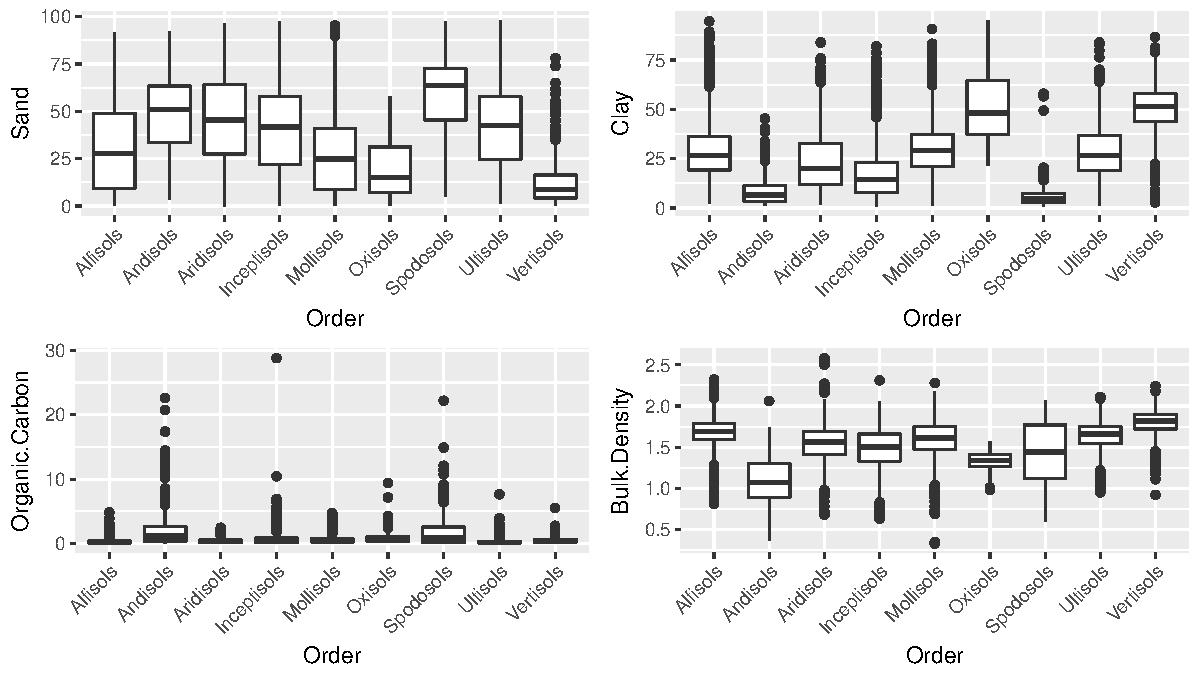
\includegraphics{Project1_files/figure-latex/EDA - Mer-1.pdf}
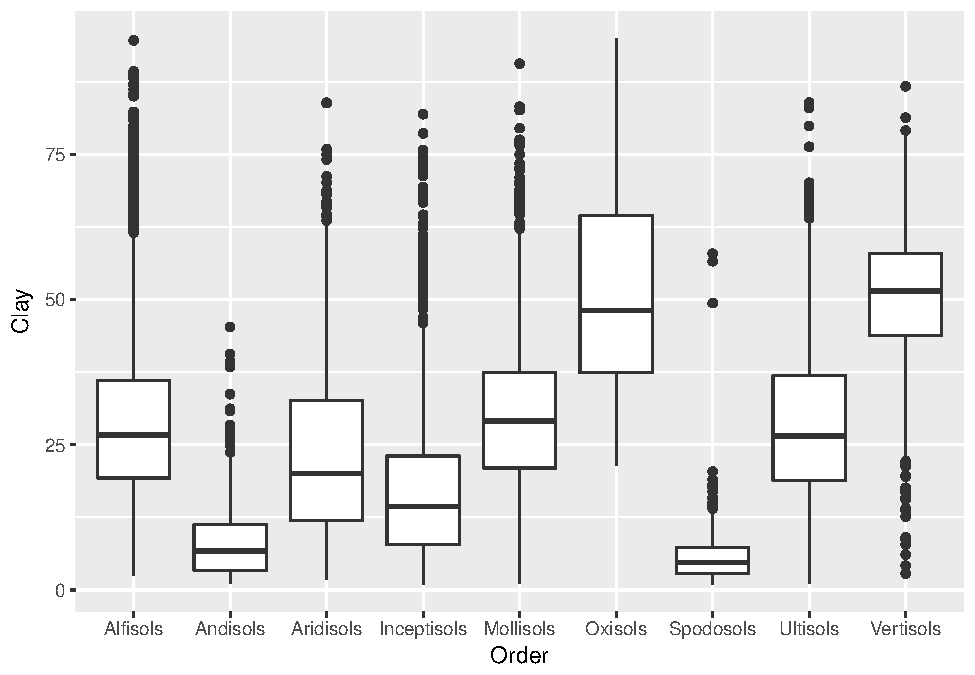
\includegraphics{Project1_files/figure-latex/EDA - Mer-2.pdf}

\section{Principle Component
Analysis}\label{principle-component-analysis}

In order to test whether dimension reduction will improve predictions we
also conducted Principle Component Analysis on the original dataset to
get a new dataset with fewer dimensions. According to our PCA results,
the first four component in total can explain about 99.8\% of variance
of the original database. The coefficients of the relevent componets are
listed in the table below. Therefore, we took the first four components
and the soil order value to build a new dataset with less dimensions.

\begin{longtable}[]{@{}lrrrr@{}}
\toprule
& PC1 & PC2 & PC3 & PC4\tabularnewline
\midrule
\endhead
Sand & 0.3516041 & 0.7770568 & -0.5154614 & 0.0820792\tabularnewline
Clay & -0.2421961 & -0.3976529 & -0.6759072 & 0.5665441\tabularnewline
Organic.Carbon & 0.0053164 & -0.0050832 & -0.0168647 &
-0.0577142\tabularnewline
Bulk.Density & -0.0019288 & 0.0000607 & -0.0029836 &
0.0104239\tabularnewline
CEC.Soil & -0.1781833 & -0.1804817 & -0.5190661 &
-0.8044793\tabularnewline
CEC.Clay & 0.0112285 & 0.0059963 & -0.0252571 &
-0.1423157\tabularnewline
Base.Saturation & -0.8859172 & 0.4526640 & 0.0839830 &
0.0374301\tabularnewline
pH & -0.0309674 & 0.0226877 & 0.0059155 & -0.0030852\tabularnewline
\bottomrule
\end{longtable}

\section{Analysis}\label{analysis}

In the following analysis with three methods (LDA, QDA and logistic) and
two datasets (original and dimension-reduced), we randomly selected 80\%
of the entire data as training data and the rest 20\% as test data.

\subsection{Linear Discriminant Analysis
(LDA)}\label{linear-discriminant-analysis-lda}

\subsubsection{Original Dataset}\label{original-dataset}

We initially conducted the LDA on the original dataset and found that
the overall prediction accuracy of our model in testing data is about
58\%. Considering we have in total 9 possible classes, the accuracy rate
is fairly good.

In the follow plots, we shows the differenced between the true and
predicted classes (top and bottom plots, respectively). It can be seen
that in the left part of the true class, there is a lot of overlap and
in the middle part, there is some overlap. But in the prediction plot,
different classes separate pretty well from each other, which indicates
that our model seperate the classes more than it should be. This overlap
between classes in reality also suggests us that we should consider more
variables to separate them well.

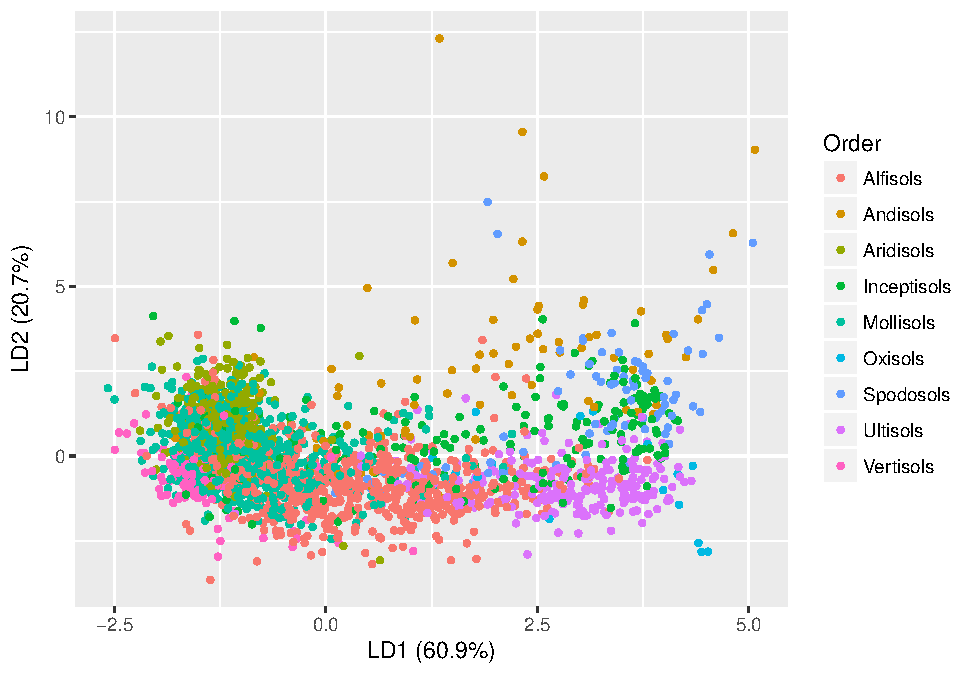
\includegraphics{Project1_files/figure-latex/lda vis - FEI-1.pdf}
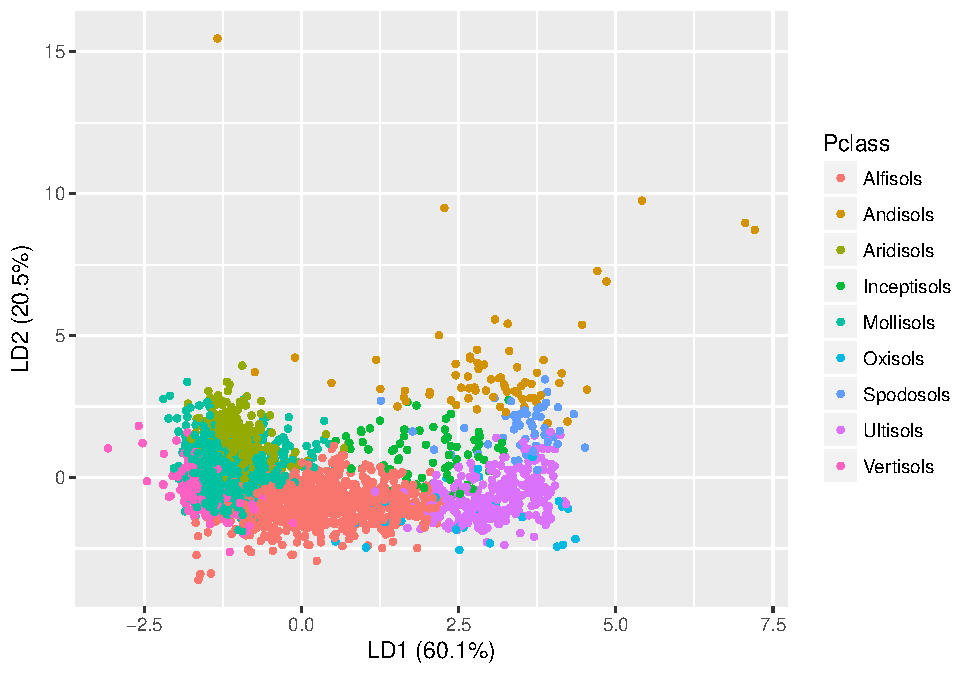
\includegraphics{Project1_files/figure-latex/lda vis - FEI-2.pdf}

\subsubsection{Reduced-Dimension
Dataset}\label{reduced-dimension-dataset}

We also conducted the same LDA method on the dimension-reduced database.
However, the result is less satisfying than using the original database.
The prediction accuracy here is about 54\%, less than 58\% of the
original database. The plot below shows the difference between the true
and predicted classes. Again, the overlap in the true class plots
indicate the difficulty to classify those samples.

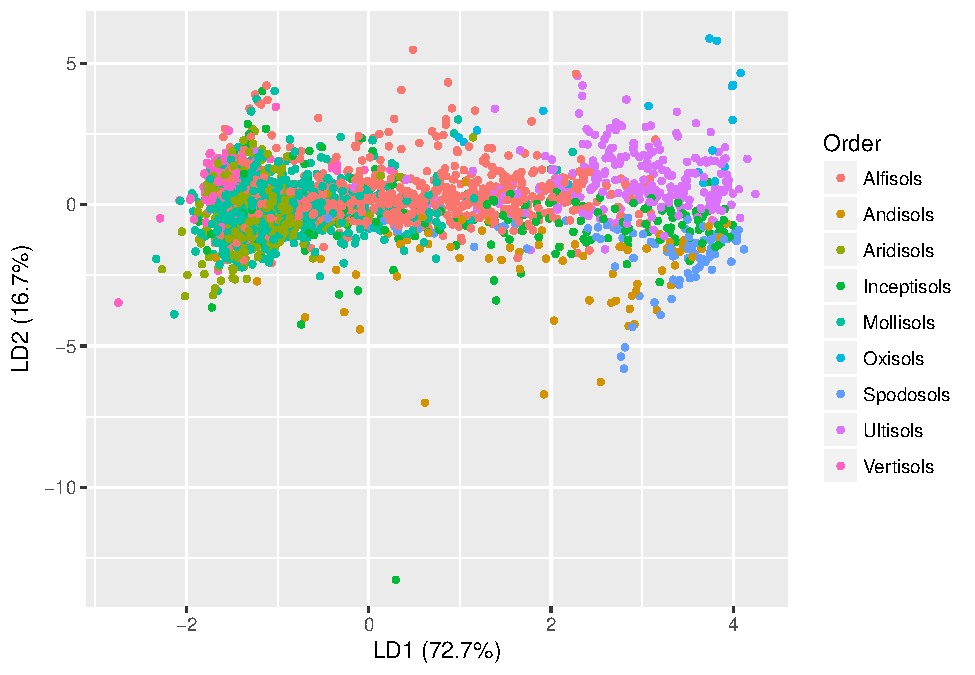
\includegraphics{Project1_files/figure-latex/LDA with PCA - Fei-1.pdf}
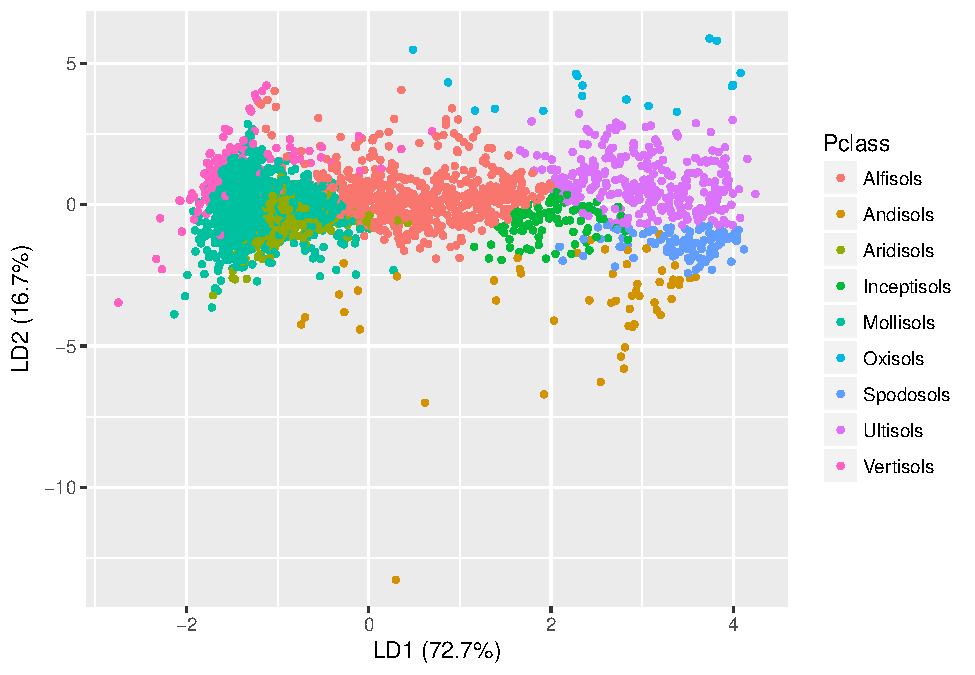
\includegraphics{Project1_files/figure-latex/LDA with PCA - Fei-2.pdf}

In the table below we can see the prediciton accuracy for each soil
Order. We can see that for most, but not all, individual soil orders the
LDA method applied to a full-dimension dataset provides the highest
percent prediciton accuracy.

\subsection{Quadratic Discriminant Analysis
(QDA)}\label{quadratic-discriminant-analysis-qda}

We used the same original and dimension-reduced dataset to apply QDA
method. The prediction accuracy of QDA is very similar to LDA. For the
original dataset, the overall accuracy is 59\%. When applying the same
method to the dimension-reduced dataset, the oveall accuracy decreases
to 57\%.

\begin{longtable}[]{@{}lrrrrrrrrr@{}}
\toprule
& Alfisols & Andisols & Aridisols & Inceptisols & Mollisols & Oxisols &
Spodosols & Ultisols & Vertisols\tabularnewline
\midrule
\endhead
QDA & 74 & 38 & 59 & 20 & 49 & 82 & 49 & 86 & 68\tabularnewline
QDA w/ PCA & 56 & 27 & 69 & 9 & 59 & 35 & 60 & 83 & 58\tabularnewline
\bottomrule
\end{longtable}

\subsection{Multinomial Logistic
Regression}\label{multinomial-logistic-regression}

Recall that the response variable for these data is an independent
9-level categorical response. With this response variable in mind, we
used the same original and dimension-reduced dataset to apply
Multinomial Logistic Regression method. The prediction accuracy again is
similar to LDA and QDA, albeit with a slight improvement. For the
original dataset, the overall accuracy is 61\%. When applying the same
method to the dimension-reduced dataset, the oveall accuracy decreases
to 58\%.

\begin{longtable}[]{@{}lrrrrrrrrr@{}}
\toprule
& Alfisols & Andisols & Aridisols & Inceptisols & Mollisols & Oxisols &
Spodosols & Ultisols & Vertisols\tabularnewline
\midrule
\endhead
MLR & 68 & 42 & 59 & 25 & 64 & 59 & 53 & 76 & 58\tabularnewline
MLR w/ PCA & 64 & 36 & 53 & 10 & 70 & 24 & 63 & 78 & 32\tabularnewline
\bottomrule
\end{longtable}

\section{Results}\label{results}

In order to compare the reults it is important to recall the diffences
between these three classification approaches. The difference between
LDA and logistic regression is that linear coefficients are estimated
differently. MLE for logistic models and estimated mean and variance
based on Gaussian assumptions for the LDA. LDA makes more restrictive
Gaussian assumptions and therefore often expected to work better than
logistic models IF they are met. QDA serves as a compromise between
non-parametric methods (not explored in this project) and the linear LDA
and logistic regression approaches. Since QDA assumes a quadratic
decision boundary, it can accurately model a wider range of problems
than can the linear methods. QDA can perform better in the presence of a
limited number of training observations because it does make some
assumptions about the form of the decision boundary.

The results from these three approaches show that the Multinomial
Logistic Regression out performed both LDA and QDA. This is likely due
to not meeting the LDA's normality assumption in addition to having a
very large dataset for testing/training.

\begin{longtable}[]{@{}lrrrrrrrrrr@{}}
\toprule
& Alfisols & Andisols & Aridisols & Inceptisols & Mollisols & Oxisols &
Spodosols & Ultisols & Vertisols & Overall\tabularnewline
\midrule
\endhead
LDA & 0.65 & 0.45 & 0.58 & 0.12 & 0.65 & 0.59 & 0.35 & 0.81 & 0.56 &
0.60\tabularnewline
QDA & 0.74 & 0.38 & 0.59 & 0.20 & 0.49 & 0.82 & 0.49 & 0.86 & 0.68 &
0.58\tabularnewline
MLR & 0.68 & 0.42 & 0.59 & 0.25 & 0.64 & 0.59 & 0.53 & 0.76 & 0.58 &
0.61\tabularnewline
\bottomrule
\end{longtable}

\section{Contributions}\label{contributions}

The different tasks required to complete this project were equally
divided between Meridith and Fei. LDA and QDA analyses were completed by
Fei while Meridith was responsible for MLR and model comparisons. Both
members of this group contributed to the presentation slides and this
report.


\end{document}
